\chapter{List-based Query Processing}
\label{list-based-processing}

In this chapter, we briefly review the traditional Volcano-style query processing technique, which is common across a wide range of different database management systems, and the column- or vector-oriented processing technique that is particularly suited for column-oriented relational database management systems. We then describe the limitations of these techniques for GDBMSs and propose a technique that we call list-based processing, that is a hybrid between the two.

\section{Existing Techniques}
\label{sec:existing-techniques}
In the Volcano-style query processors~\cite{volcano} execution happens by passing a single tuple between operators. Specifically, each operator operates on a single intermediate tuple, e.g., a partial match of the subgraph query,  extends or modifies one value in this tuple and passes it to the next operator in the query plan.  Consider the following query and a plan for this query shown in Figure~\ref{fig:proc-qp}.

\begin{example}
	\label{ex:proc-example}
	Consider the following query. 
	{\em 
		\begin{lstlisting}[numbers=none,  showstringspaces=false,belowskip=0pt ]
		MATCH (a:PERSON)$-$[ex:FOLLOWS]$\rightarrow$(b:PERSON),
		$\qquad\quad$(b:PERSON)$-$[ey:FOLLOWS]$\rightarrow$(c:PERSON)
		WHERE a = $v_4$
		RETURN ey.since\end{lstlisting}
	}
\end{example}

 In a GDBMS that adopts the Volcano-style processing, a scan operator could match the $a$ variable to $v_4$  then give the partial match $[a=v_4]$ to the next join operator $jo_1$. Suppose $v_4$ has $k$ many outgoing edges, say $(e_{41}, v_{41}), ..., (e_{4k}, v_{4k})$. $jo_1$ would read the first edge $(e_{41}, v_{41})$ and give the tuple $[a=v_4, e_x=e_{41}, b=v_{41}]$ to the next join operator $jo_2$. $jo_2$ would then read the first outgoing edge of $v_{41}$, say $(e_{411}, v_{411})$, and give the tuple  $[a=v_4, e_x=e_{41}, b=v_{41}, e_y=e_{411}, c=v_{411}]$ to the next property reader operator, so and so forth. One advantage of Volcano-style processing is that even if there are many intermediate tuples with a particular variable  value, this value is copied only once to the tuple that is passed between operators. For example, even if $v_{41}$ has $z_1$ many outgoing edges in the input graph, so there will be $z_1$ many intermediate tuples with $b=v_{41}$, this value is copied to the tuple only once. This is an important advantage for GDBMSs where 1-to-many joins, specifically one vertex joining to many neighbor vertices are common.   At the same time, it is well known that Volcano-style processors do not achieve high CPU cache locality. For example although $(e_{41}, v_{41}), ...., (e_{4k}, v_{4k})$ are stored consecutively in memory, reading and processing these values are intermixed with function calls to the other operators which might read values from other adjacency lists. The second shortcoming of Volcano-style processors is that they perform many function calls between operators.

\vspace{-5pt}

\begin{figure}
	\begin{center}
		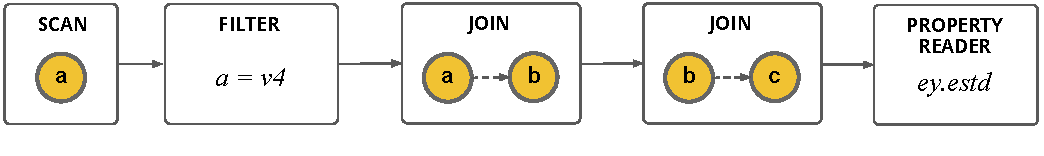
\includegraphics[scale=0.78]{img/proc-qp}
	\end{center}
		\caption{Query plan for Example~\ref{ex:proc-example}.}
	\label{fig:proc-qp}
\end{figure}

Column-oriented relational systems have addressed the shortcomings of Volcano-style processors by introducing column- and vector-oriented processing~\cite{boncz-phd, monet-2decades}. Instead of a tuple-at-a-time processing, these techniques pass an entire column or vector, e.g., 1024 tuples, at a time between operators. Each primitive operator in the system takes a vector of tuples and outputs a vector of tuples. 
While processing a vector, each operator can read consecutive memory locations, achieving good cache locality, and employ efficient block algorithms and tight loop over arrays that draw benefits from advanced compiler optimizations and SIMD instructions that are common in modern CPUs. Vector-at-a-time processing also reduces the number of function calls that are made during query processing. One shortcoming of vector-oriented processing is that, for 1-to-many joins, it requires copying intermediate values. For example in a vector-oriented processor, the scan operator would output $a:[v_4]$ vector, the first join operator $jo_1$ would output $a:[v_4, v_4, ...., v_4]$, $e_x:[e_{41}, ..., e_{4k}]$, $b:[v_{41}, ..., v_{4k}]$ vectors, and the second join operator $jo_2$ would output  $a:[v_4, v_4, ...., v_4]$, $e_x:[e_{41},...,e_{41}, e_{42}, ..., e_{42}, ...., e_{4k}, e_{4k}]$, $b:[v_{41},...,v_{41}, v_{42}, ..., v_{42}, ...., v_{4k}, v_{4k}]$, $e_y:[e_{411},...,e_{41z_1}, e_{421}, ..., e_{42z_2}, ...., e_{4k1}, e_{4kz_k}]$, $c:[v_{411},...,v_{41z_1}, v_{421}, ..., v_{42z_2}, ...., v_{4k1}, v_{4kz_k}]$, assuming vertices $v_{41}$, $v_{42}$, ..., $v_{4k}$ have $z_1$, ..., $z_k$ neighbors, respectively (and assuming $z_1 +  ..., + z_k$ is less than the fixed vector size). While vector style processing is good for aggregation heavy workloads that require reading columns of data consecutively, it is not particularly suited for workloads that contain many 1-to-many joins due to the data duplication it requires.


\section{List-based Processing}
\label{sec:list-based-proc}

We have developed a new query processing technique, that we call, {\em list-based processing} that is a hybrid between Volcano-style and vector-oriented processing. In particular we have two versions of each operator, a Volcano-style and a vector-oriented version. For example, we have a \texttt{JOIN} operator that takes an intermediate tuple and copies one value of one adjacency list and produces one tuple. We also have a \texttt{LIST JOIN} operator that takes a tuple and produces an output tuple that contains a copy of an adjacency list that is used in extending. We do lazy evaluation so until it is necessary, the list is simply a pointer to the adjacency list that should be extended and is not materialized. Similarly we have a \texttt{PROPERTY READER} and \texttt{LIST PROPERTY READER} operators, where the latter takes a tuple where one value is an adjacency list containing a list of edges and neighbors, and copies over a property of the edges or neighbors. For example, Figure~\ref{fig:proc-lbqp} shows the query plan that operates on lists rather than single values. The last join operator is \texttt{LIST JOIN} followed by the \texttt{LIST PROPERTY READER} for reading property of $e_y$ edge matches. The execution is performed Volcano-style until the \texttt{LIST-JOIN} operator, which for example would get the tuple $[a=v_4, b=v_{41}]$, and outputs $[a=v_4, b=v_{41}, c=\{(e_{411}, v_{411}), ..., (e_{41z_1}, v_{41z_1})\}]$ as output. The \texttt{LIST PROPERTY READER} could then output  $[a=v_4, b=v_{41}, c=\{(e_{411}, v_{411}), ..., (e_{41z_1}, v_{41z_1})\}, e_y=\{1980, 1981, ...., 1990\}]$. 

The list operators perform vector-oriented processing with tight loops but the vector size is not fixed and is the size of one adjacency list. For example, the \texttt{LIST PROPERTY READER} would directly access a property page and read all of the properties of $e_{411}, ..., e_{41z_1}$ inside a single loop. The \texttt{LIST JOIN} operator and the following list operators are only used when no other \texttt{JOIN} operator needs to extend the values in the list produced by \texttt{LIST JOIN}. For example \texttt{LIST JOIN} is used in the final join operators in a plan, e.g., $jo_2$ in our example, but it can also be used in earlier join operators, as long as the output list of \texttt{LIST JOIN} will not be extended in another join operator. The final plans therefore consists of a mix of Volcano- and vector-oriented operators. Similar to Volcano-style processing, list-based processing does not copy the same value into the tuple multiple times and also benefits from vector-oriented processing, specifically for the operators that are at the leaves of the query plans. We note that in many queries, most of the work is done by the join operators in the leaf, so an important part of the processing is often still performed in a vector-oriented style. As we will demonstrate in Chapter~\ref{c:evaluation}, list-oriented processing can outperform both Volcano-style and vector-oriented processing. This is especially the case when queries contain multiple 1-to-many joins, corresponding to multi-hop traversals of graphs.

We note that our list-oriented processing is a simple form of {\em factorized query processing}~\cite{olteanu}, that evaluate queries in a compressed format. For example, the tuple  $[a=v_4, b=v_{41}, c=\{(e_{411}, v_{411}), ..., (e_{41z_1}, v_{41z_1})\}, e_y=\{1980, 1981, ...., 1990\}]$ is a compressed representation of $z_1$ many tuples. For some queries, e.g., a star query, this type of processing can significantly decrease the amount of intermediate data that is processed. A rigorous study of factorized query processing in GDBMSs is not in the scope of this thesis and is left for future work.

\begin{figure}
	\hfill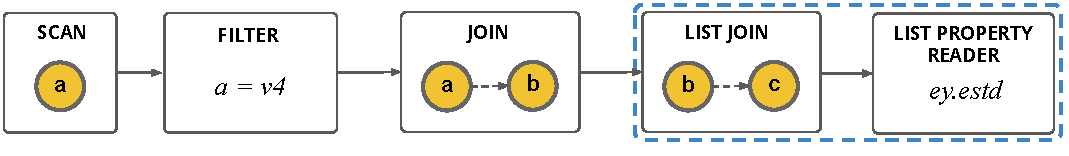
\includegraphics[scale=0.78]{img/proc-lbqp}\hfill
	\vspace{-10pt}
	\caption{Query plan with List-based Processing for Example~\ref{ex:proc-example}.}
	\vspace{-8pt}
	\label{fig:proc-lbqp}
\end{figure}









